% Gemini theme
% https://github.com/anishathalye/gemini

\documentclass[final]{beamer}

% ====================
% Packages
% ====================

\usepackage[T1]{fontenc}
\usepackage{lmodern}
\usepackage[size=custom,width=83.82,height=60.96,scale=1.0]{beamerposter}
\usetheme{gemini} %\usecolortheme{gemini}
\usecolortheme{owl}
\usepackage{graphicx}
\usepackage{booktabs}
\usepackage{tikz}
\usepackage{amssymb}
\usepackage{amsmath}
\usepackage{pgfplots}
\usepackage{tabularx}
\usepackage{enumitem}
\usepackage{caption,amsmath,graphicx,url,amssymb,latexsym,epsfig,tabularx,setspace,multirow,threeparttable,longtable,pdflscape,tabu,comment,subfigure,textcomp,xparse}

\definecolor{darkblue}{RGB}{39, 60, 200}
\setbeamercolor{headline}{fg=lightgray,bg=darkblue}
\setbeamercolor{headline rule}{bg=darkblue}


% ====================
% Lengths
% ====================

% If you have N columns, choose \sepwidth and \colwidth such that
% (N+1)*\sepwidth + N*\colwidth = \paperwidth
\newlength{\sepwidth}
\newlength{\colwidth}
\setlength{\sepwidth}{0.010\paperwidth}
\setlength{\colwidth}{0.3\paperwidth}

\newcommand{\separatorcolumn}{\begin{column}{\sepwidth}\end{column}}

% ====================
% Control Sequences
% ====================

%\def\DtoH{\textit{DtoH}\xspace}
%\def\HtoD{\textit{HtoD}\xspace}

\def\DtoH{\textit{DtoH}}
\def\HtoD{\textit{HtoD}}

% ====================
% Title
% ====================

\title{New Title}

\author{Jordan Wright \inst{1}, Zane Fink \inst{1}, \and Michael Gowanlock\inst{1}}

\institute[shortinst]{\inst{1} School of Informatics, Computing, and Cyber Systems at Northern Arizona University}

% ====================
% Body
% ====================

\begin{document}

\begin{frame}[t]
\begin{columns}[t]
\separatorcolumn

\begin{column}{\colwidth}

  \begin{block}{Abstract}

   Many database operations have a low compute to memory access ratio where achieving performance gains is percieved as insurmountable. We examine several of these memory-bound algorithms, 
   including $(i)$ batched predecessor searches; $(ii)$ multiway merging; and, $(iii)$ partitioning. 
   We examine the performance of parallel CPU-only, GPU-only, and hybrid CPU/GPU approaches, and show 
   that hybrid algorithms achieve performance gains. We develop a model that considers 
   main memory accesses and PCIe data transfers, which are two major bottlenecks for hybrid CPU/GPU algorithms. 
   The model lets us determine how to share work between the CPU and GPU to maximize resource 
   utilization while minimizing load imbalance. We show that our model can accurately predict the fraction of work 
   to be sent to each, and thus confirms that these overlooked database primitives can be 
   accelerated. 

  \end{block}

  \begin{block}{Introduction}
    
\begin{description}[font=$\bullet$~\normalfont\scshape\color{red!50!black}]

\item While compute-intensive operations have seen performance gains using GPUs, many database primitives, which perform many operations in-memory, have not been accelerated. 

\item One approach to improve the performance of memory-bound algorithms is to develop hybrid parallel algorithms that use both CPU and GPU resources.

\item We utilize both the CPU and GPU to compute these database primitives.

\item We propose \emph{accelerating the unacceleratable} --- which we define as memory-bound database primitives that are well-suited to a hybrid CPU/GPU execution but not necessarily a GPU-only execution. 

\item Our model for both CPU and GPU performance uses the well-known external memory (EM) model with the exception that we consider the total number of main memory \emph{elements} loaded/stored as our performance metric.

\end{description}  

  \end{block}

  \begin{alertblock}{Problem Statement}
   For each of our database primitives we implement CPU-only, GPU-only, and hybrid CPU/GPU algorithms. 
   We consider a platform with multi-core CPUs and a GPU, where the total response time includes all 
   data transfers to and from the GPU and related overheads. We assume that each algorithm can exceed the GPU's global memory capacity. 
  \end{alertblock}

\end{column}

\separatorcolumn

\begin{column}{\colwidth}

 \begin{block}{Hybrid Algorithms}

 \begin{description}[font=$\bullet$~\normalfont\scshape\color{red!50!black}]
\item The three algorithms that we consider are parallelizable across both architectures while minimizing memory accesses. We accomplish this by breaking up the total work into several \emph{batches} of divisible workloads that can be computed independently on either architecture. 

\item We define $n_b$ to be the number of batches. For batched predecessor search and partitioning, we arbitrarily select $n_b=400$, while for multiway merge, we make $n_b$ a function of $k$. 

\item Let $\beta$ be the unidirectional bandwidth over PCIe, $\gamma$ be the memory bandwidth between the CPU and main memory when reading, and $\alpha$ be the memory bandwidth between the CPU and main memory when simultaneously reading and writing. For a given platform, $\beta$, $\gamma$, and  $\alpha$ can be obtained through simple microbenchmarks.

\item We obtain $\alpha=19.56$~GiB/s, $\gamma=34.01$~GiB/s, and $\beta=11$~GiB/s on our platform. 
\end{description} 

\begin{figure}[htp]
\centering
%width=0.22
    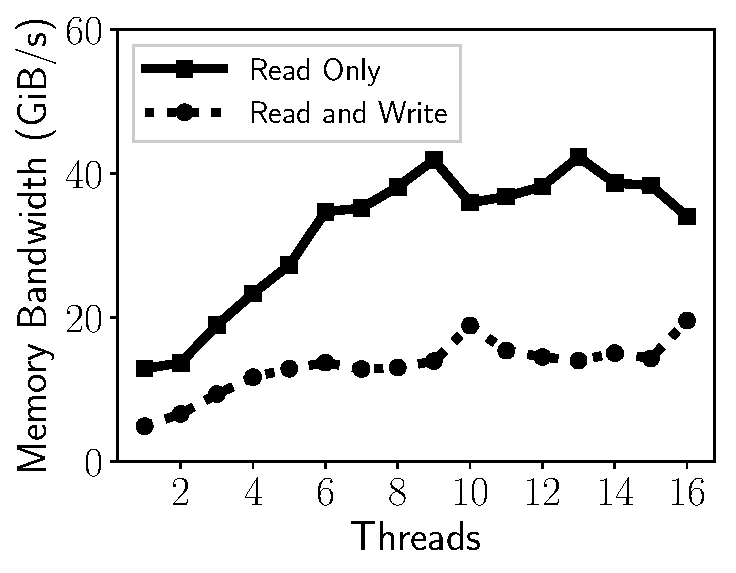
\includegraphics[height=0.2\textwidth, width=0.30\textwidth, trim={0.5cm 0.5cm 0.5cm 1cm}]{figures/microbenchmarks_time_vs_threads.pdf}	
   \label{fig:mem_bandwidth_scalability}
\end{figure}


\heading{Scan}
We define scan as follows, and use the $max$ function, which requires reading all $n$ elements in a list to find the maximum value (alternatively,
we could use a different function, such as $min$, but the complexity is the same).
Let $A$ be an unordered array of $n$ elements. We wish to find $x \in A$ such that for all $y \in A$, $x \ge y$, i.e. $x = max(A)$.


\heading{Batched Predecessor Search}
   Let $A$ be a set of keys sorted in non-decreasing order,  
   where each key is denoted as $a_i$, where $i=1, 2,\ldots,n$, and $B$ be a set of queries sorted in non-decreasing order, 
   where each query is denoted as $b_j$, where $j=1, 2,\ldots,n$. For each query, $b_j\in B$, the batched predecessor search 
   finds the largest value of $i$, such that $a_i\leq b_j$. While $A$ and $B$ can vary in size, for simplicity, we assume $|A|=|B|=n$.

\heading{Multiway Merging}

   Given input array $A$ consisting of $k$ sublists, denoted as $S_j$, 
   where $j=1, 2,\ldots,k$, each of size  $\frac{n}{k}$ and sorted in non-decreasing order, we wish to output the $n$ total elements 
   in sorted order. Furthermore, we assume that $k$ is small enough that we can load elements 
   from each sublist into memory without degrading CPU cache utilization.

  \end{block}

\end{column}

\separatorcolumn

\begin{column}{\colwidth}

  \begin{block}{Research Highlights}
\begin{figure}[htp]
\centering
\subfigure[]{
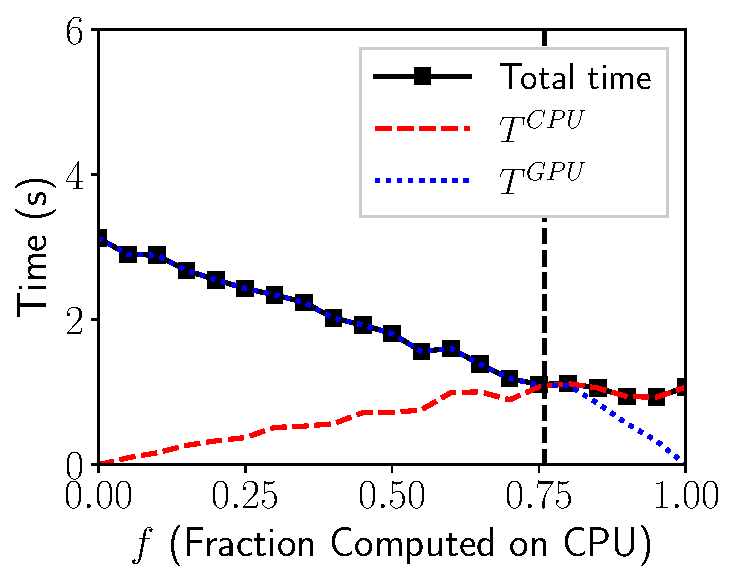
\includegraphics[height=0.25\textwidth, width=0.3\textwidth, trim={0.2cm 0.2cm 0.2cm 0.2cm}]{figures/time_vs_cpu_frac_scan.pdf}
}
\subfigure[]{
    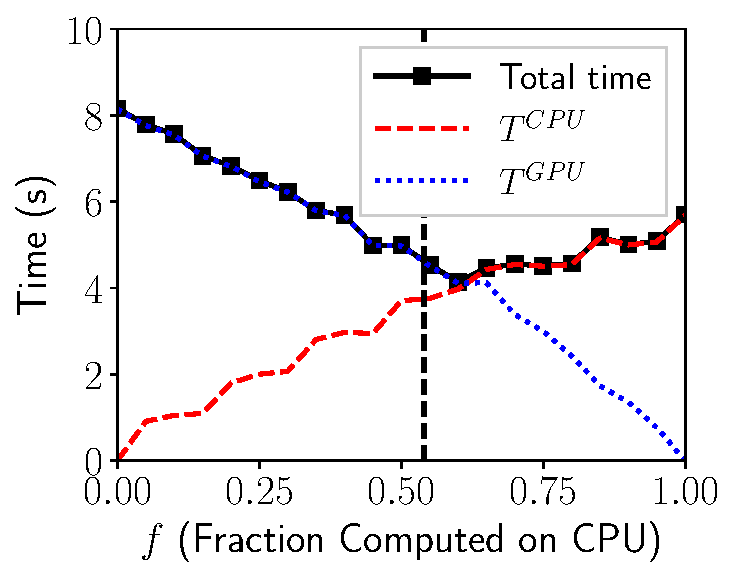
\includegraphics[height=0.25\textwidth, width=0.3\textwidth, trim={0.2cm 0.2cm 0.2cm 0.2cm}]{figures/time_vs_cpu_frac_predecessor.pdf}     
    }
\subfigure[]{
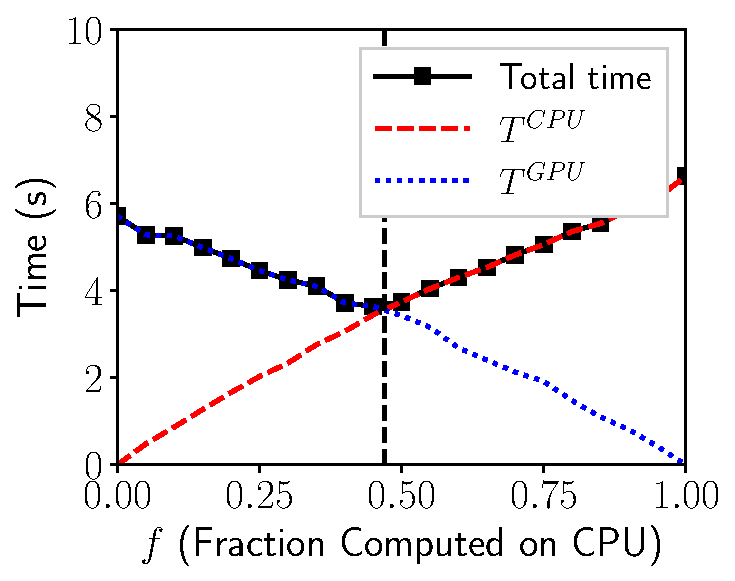
\includegraphics[height=0.25\textwidth, width=0.3\textwidth, trim={0.2cm 0.2cm 0.2cm 0.2cm}]{figures/time_vs_cpu_frac_multiway.pdf}}

%\captionsetup[figure]{font=small}
 \caption{Hybrid model accuracy for the scan, batched predecessor search, and multiway merging. The total response time, $T^{CPU}$, and $T^{GPU}$ vs. $f$, are plotted. We show $n=4.0\times10^9$ for all algorithms. The vertical dashed line in each plot denotes the modeled value of $f$.}

 \label{fig:time_vs_f}
\end{figure}

\begin{description}[font=$\bullet$~\normalfont\scshape\color{red!50!black}]
\item Figure 2(a) demonstrates that the model accurately predicts $f$ for the scan ($f=0.76$).
\item  Figure2(b) indicates that the model's prediction is quite accurate for multiway merging ($f=0.47$).
\item  Figure 2(c) shows that even if the model can predict a good value for $f$, small differences in $f$ can yield significant load imbalance ($f=0.35$). 
\end{description}

%trim={0.2cm 0.2cm 0.2cm 0.2cm}
 \begin{figure}[htp]
\centering
\subfigure[]{
    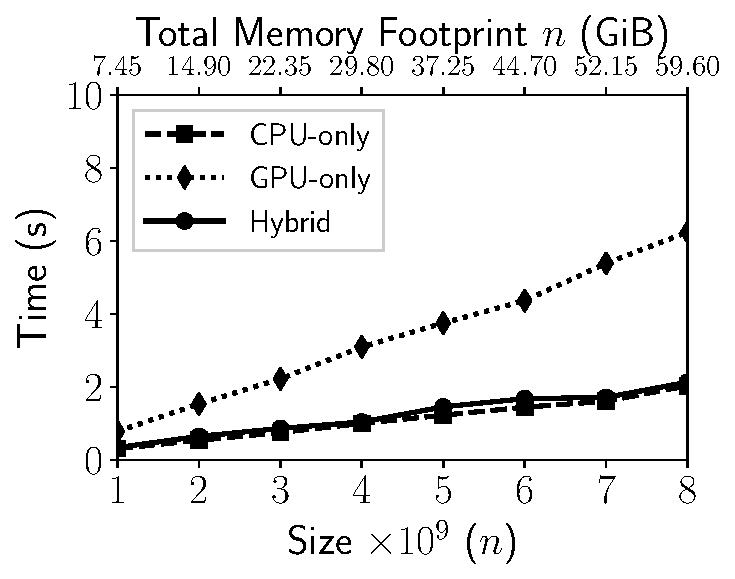
\includegraphics[height = 0.25\textwidth, width=0.30\textwidth, trim={0.2cm 0.2cm 0.2cm 0.2cm}]{figures/size_vs_time_linear_scan.pdf}	
}
\subfigure[]{
    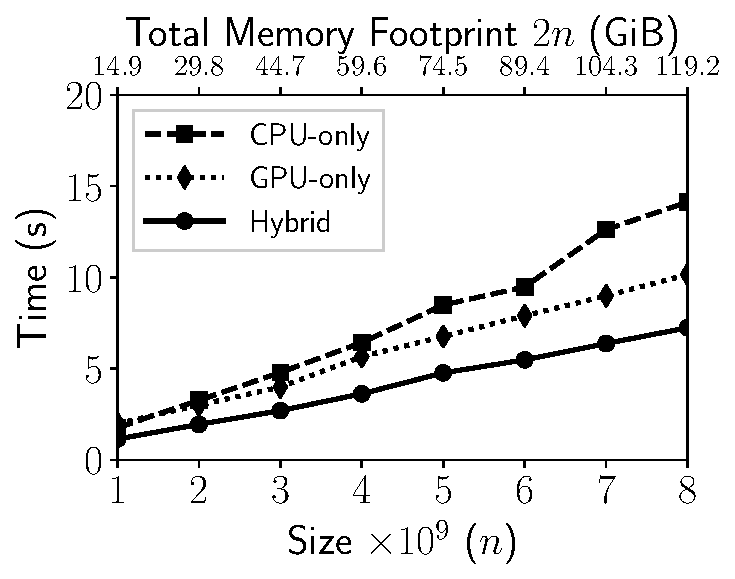
\includegraphics[height=0.25\textwidth, width=0.30\textwidth, trim={0.2cm 0.2cm 0.2cm 0.2cm}]{figures/size_vs_time_multiway.pdf}	
}
\subfigure[]{
    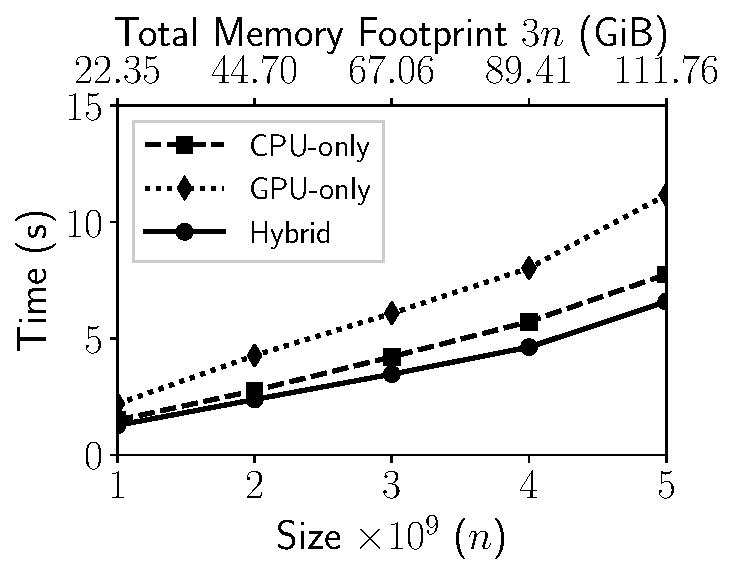
\includegraphics[height=0.25\textwidth, width=0.30\textwidth, trim={0.2cm 0.2cm 0.2cm 0.2cm}]{figures/size_vs_time_predecessor.pdf}	
}
   \caption{CPU-Only, GPU-Only and Hybrid runtimes for the scan (a), multiway merging (b), and batched predecessor search (c).}
   \label{fig:predecessor_search_results}
\end{figure}

\end{block} 
\begin{description}[font=$\bullet$~\normalfont\scshape\color{red!50!black}]
\item We find that the hybrid model achieves a speedup over both the CPU-Only and GPU-Only times for the batched predecessor search and multiway merging $n$. 
\item However, the overheads associated with the hybrid algorithm for the scan result in a slowdown.
\end{description}


\begin{block}{Future Work}

\begin{description}[font=$\bullet$~\normalfont\scshape\color{red!50!black}]
\item Investigating whether compression schemes or other memory transfer optimizations can alleviate some of the bottlenecks, despite the computational overhead.
\item The study of other fundamental database operations that have not been considered for GPU acceleration.
\end{description}

\end{block}

\begin{block}{Acknowledgements}
This material is based upon work supported by the National Science Foundation under Grant OAC-1849559 and Fonds de la Recherche Scientifique-FNRS under Grant no MISU F 6001 1.
\end{block}

\end{column}

\separatorcolumn
\end{columns}
\end{frame}

\end{document}
